% % XeLaTeX document
% \documentclass[12pt,a4paper]{article}

% % Редактируем: конфигурация, личные настройки: имя, название предмета и пр. для титульной страницы и метаданных документа здесь
% \newcommand{\university}{Санкт-Петербургский политехнический университет Петра Великого}
\newcommand{\faculty}{Институт физики, нанотехнологий и телекоммуникаций}
\newcommand{\department}{Высшая инженерно-физическая школа}
\newcommand{\city}{Санкт-Петербург}
\newcommand{\num}{}
\newcommand{\docname}{Отчет по лабораторной работе №1}
\newcommand{\subject}{Молекулярное моделирование}
\newcommand{\tutorname}{И. М. Соколов}
\newcommand{\studentname}{В. Х. Салманов}
\newcommand{\group}{3430302/60201}

% % Не редактируем: используемые пакеты
% % настройка кодировки, шрифтов и русского языка
\usepackage{fontspec}
\usepackage{polyglossia}

% рабочие ссылки в документе
\usepackage{hyperref}

% графика
\usepackage{graphicx}
\usepackage{tikz}

% поворот страницы
\usepackage{pdflscape}

% качественные листинги кода
\usepackage{minted}
\usepackage{listings}
\usepackage{lstfiracode}

% отключение копирования номеров строк из листинга, работает не во всех просмотрщиках (в Adobe Reader работает)
\usepackage{accsupp}
\newcommand\emptyaccsupp[1]{\BeginAccSupp{ActualText={}}#1\EndAccSupp{}}
\let\theHFancyVerbLine\theFancyVerbLine
\def\theFancyVerbLine{\rmfamily\tiny\emptyaccsupp{\arabic{FancyVerbLine}}}

% библиография
\bibliographystyle{templates/gost-numeric.bbx}
\usepackage{csquotes}
\usepackage[parentracker=true,backend=biber,hyperref=false,bibencoding=utf8,style=numeric-comp,language=english,autolang=other,citestyle=gost-numeric,defernumbers=true,bibstyle=gost-numeric,sorting=ntvy,]{biblatex}

% установка полей
\usepackage{geometry}

% нумерация картинок по секциям
\usepackage{chngcntr} 

% дополнительные команды для таблиц
\usepackage{booktabs}

% для заголовков
\usepackage{caption} 
\usepackage{titlesec}
\usepackage[dotinlabels]{titletoc}

% разное для математики
\usepackage{amsmath, amsfonts, amssymb, amsthm, mathtools}
\usepackage{braket}


% водяной знак на документе, см. main.tex
\usepackage[printwatermark]{xwatermark} 

% использование различных спец. символов
\usepackage{gensymb}

% таблицы
\usepackage{tabularx}
\newcolumntype{Y}{>{\centering\arraybackslash}X}

% гиперссылки
\usepackage{hyperref}

% межстрочный интервал
\sloppy
\linespread{1.2}
\usepackage{multirow}
\usepackage{graphicx}

\usepackage{import}

% % Не редактируем: параметры используемых пакетов и не только
% % настройки polyglossia
\setdefaultlanguage{russian}
\setotherlanguage{english}

% локализация
\addto\captionsrussian{
  \renewcommand{\figurename}{Рисунок}%
  \renewcommand{\partname}{Глава}
  \renewcommand{\contentsname}{\centerline{Содержание}}
  \renewcommand{\listingscaption}{Листинг}
}

% основной шрифт документа
\setmainfont{CMU Serif}

% перечень использованных источников
\addbibresource{refs.bib}

% настройка полей
\geometry{top=2cm}
\geometry{bottom=2cm}
\geometry{left=3cm}
\geometry{right=1.5cm}
\geometry{bindingoffset=0cm}

% настройка ссылок и метаданных документа
\hypersetup{unicode=true,colorlinks=true,linkcolor=red,citecolor=green,filecolor=magenta,urlcolor=cyan,
    pdftitle={\docname},   	    
    pdfauthor={\studentname},      
    pdfsubject={\subject},      		        
    pdfcreator={\studentname}, 	       
    pdfproducer={Overleaf}, 		     
    pdfkeywords={\subject}
}

% настройка подсветки кода и окружения для листингов
\usemintedstyle{colorful}
\newenvironment{code}{\captionsetup{type=listing}}{}

% шрифт для листингов с лигатурами
\setmonofont{FiraCode-Regular.otf}[
    Path = templates/,
    Contextuals=Alternate
]

% оформления подписи рисунка
\captionsetup[figure]{labelsep = period}

% подпись таблицы
\DeclareCaptionFormat{hfillstart}{\hfill#1#2#3\par}
\captionsetup[table]{format=hfillstart,labelsep=newline,justification=centering,skip=-10pt,textfont=bf}

% путь к каталогу с рисунками
\graphicspath{{fig/}}

% Внесение titlepage в учёт счётчика страниц
\makeatletter
\renewenvironment{titlepage} {
 \thispagestyle{empty}
}
\makeatother

\counterwithin{figure}{subsection}
\counterwithin{table}{subsection}

\titlelabel{\thetitle.\quad}

% для удобного конспектирования математики
\mathtoolsset{showonlyrefs=true}
\theoremstyle{plain}
\newtheorem{theorem}{Теорема}[subsection]
\newtheorem{proposition}[theorem]{Утверждение}
\theoremstyle{definition}
\newtheorem{corollary}{Следствие}[theorem]
\newtheorem{problem}{Задача}[subsection]
\theoremstyle{remark}
\newtheorem*{nonum}{Решение}

% настоящее матожидание
\newcommand{\MExpect}{\mathsf{M}}

% объявили оператор!
\DeclareMathOperator{\sgn}{\mathop{sgn}}

% перенос знаков в формулах (по Львовскому)
\newcommand*{\hm}[1]{#1\nobreak\discretionary{} {\hbox{$\mathsurround=0pt #1$}}{}} 

% формулы
\newcommand{\mequation}[1]{
\begin{equation}
\begin{split}
\begin{gathered}
#1
\end{gathered}
\end{split}
\end{equation}
}

% % водяной знак для обозначения статуса документа
% %\newwatermark[allpages,color=red!40,angle=45,scale=3,xpos=0,ypos=0]{DRAFT}

% \begin{document}
% % Не редактируем: Титульная страница (формируется автоматически из заданной конфигурации)
% \begin{titlepage}	% начало титульной страницы

	\begin{center}		% выравнивание по центру

		\large \university \\
		\large \faculty \\
		\large \department \\[5cm]
		% название института, затем отступ 6см
		
		\LARGE \textbf \subjecttype \\ % тип работы (например: курсовая работа)
		\LARGE \subject \\[0.5cm] % название работы, затем отступ 0,5см
		\large \docname \num \\[4.1cm]
		%\large Тема работы\\[5cm]

	\end{center}


	\begin{flushright} % выравнивание по правому краю
		\begin{minipage}{0.25\textwidth} % врезка в половину ширины текста
			\begin{flushleft} % выровнять её содержимое по левому краю

				\large\textbf{Работу выполнил:}\\
				\large \studentname \\
				\large {Группа:} \group \\
				
				\large \textbf{Преподаватель:}\\
				\large \tutorname

			\end{flushleft}
		\end{minipage}
	\end{flushright}
	
	\vfill % заполнить всё доступное ниже пространство

	\begin{center}
	\large \city \\
	\large \the\year % вывести дату
	\end{center} % закончить выравнивание по центру

\end{titlepage} % конец титульной страницы

\vfill % заполнить всё доступное ниже пространство


% % Не редактируем: Страница содержания (формируется автоматически из section, subsection и пр., указанных в content.tex)
% % Содержание
\setcounter{tocdepth}{1} % Show sections
\setcounter{tocdepth}{2} % + subsubsections
\setcounter{tocdepth}{3} % + paragraphs
\setcounter{tocdepth}{4} % + paragraphs
\setcounter{tocdepth}{5} % + subparagraphs
\tableofcontents
\newpage



% % Редактируем: всё остальное: вступление, др. этапы, заключение, приложение
\subsection{Цель работы}
Определить возможные структуры комплексов пропанола с молекулой воды и энергии образующейся при этом водородной связи.


\subsection{Постановка задач}
Предположить возможные комплексы молекул пропанола с водой, провести оптимизацию методом RHF/STO-3G и привести следующие результаты: 
\begin{itemize}
    \item число действительно различных комплексов с водородной связью;
    \item для каждого комплекса -- энергию водородной связи;
    \item наиболее энергетически выгодный комплекс и соответствующее значение водородной связи.
\end{itemize}

\begin{figure}[H]
\centering
\captionsetup{justification=centering}
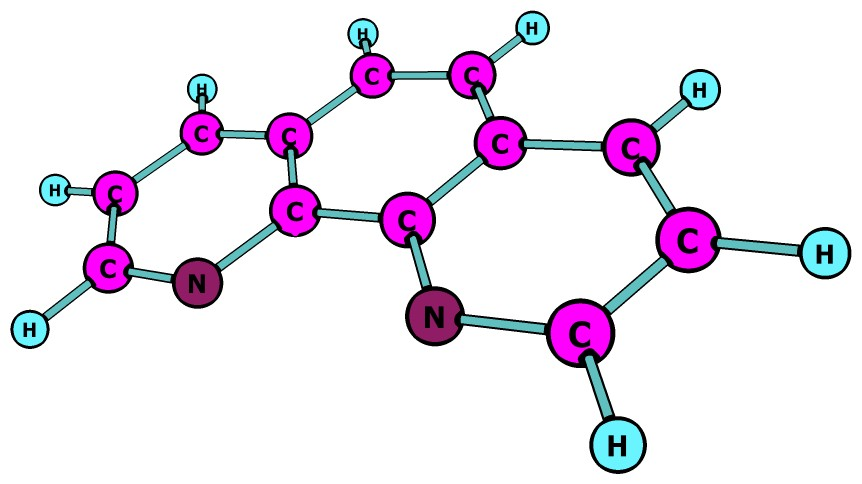
\includegraphics[scale=0.4]{fig/0.jpg}
\caption{Один из предложенных комплексов пропанола с молекулой воды.}
\end{figure}


\subsection{Теоретическая информация}
\subsubsection{Водородная связь}
Водородная связь — форма ассоциации между электроотрицательным атомом и атомом водорода H, связанным ковалентно с другим электроотрицательным атомом. В качестве электроотрицательных атомов могут выступать N, O или F. Энергия водородной связи, как правило, по абсолютной величине находится в пределах (0.003 - 0.022) Хартри.

\begin{figure}[H]
\centering
\captionsetup{justification=centering}
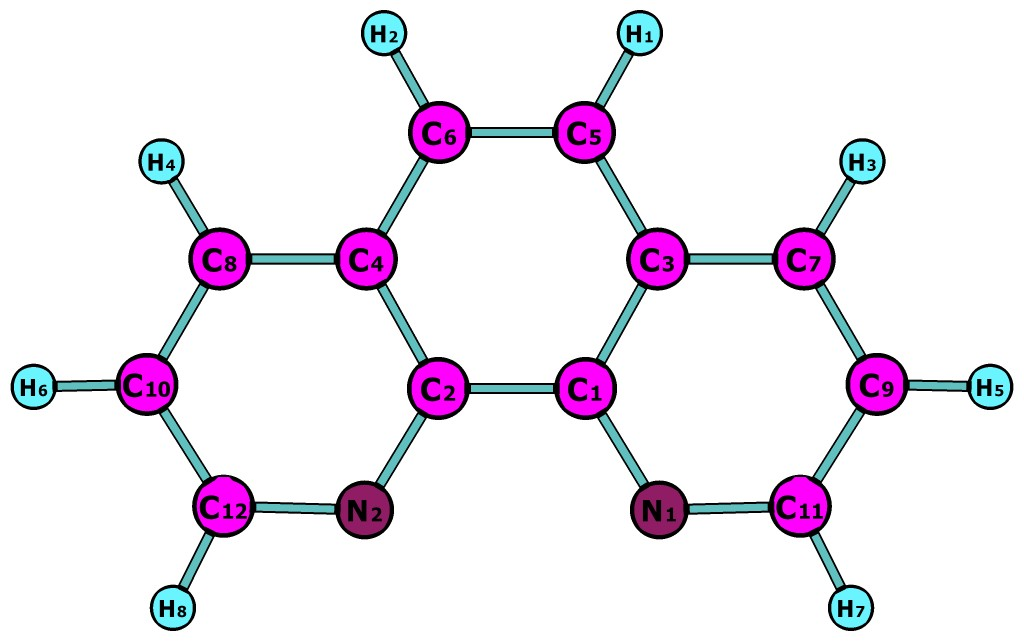
\includegraphics[scale=0.2]{fig/1.jpg}
\caption{Водородная связь между молекулами воды (чёрные пунктирные линии).}
\end{figure}


\subsection{Результаты}
Было предложено 5 различных комплексов. После проведения оптимизации были получены два стабильных различных комплекса. Информация о данных комплексах приведена в таблице ниже: 

\begin{table}[H]
\caption{Составляющие энергии комплексов} \label{tab:my-table}
\begin{center}
\resizebox{\textwidth}{!}{%
\begin{tabular}{|c|c|c|c|c|}
\hline
№ комплекса & Описание комплекса & \begin{tabular}[c]{@{}c@{}}Полная энергия\\ комплекса, Хартии\end{tabular} & \begin{tabular}[c]{@{}c@{}}Полная энергия \\ невзаимодействующего\\ комплекса, Хартри\end{tabular} & \begin{tabular}[c]{@{}c@{}}Энергия водородной\\ связи, Хартии\end{tabular} \\ \hline
1 & \begin{tabular}[c]{@{}c@{}}Водородная связь между\\ O2 и H1\end{tabular} & -265.688 & -265.678 & 0.01 \\ \hline
2 & \begin{tabular}[c]{@{}c@{}}Водородная связь между\\ O1 и H3\end{tabular} & -265.687 & -265.678 & 0.009 \\ \hline
\end{tabular}%
}
\end{center}
\end{table}

Более стабильным оказался первый комплекс.

\begin{figure}[H]
\centering
\captionsetup{justification=centering}
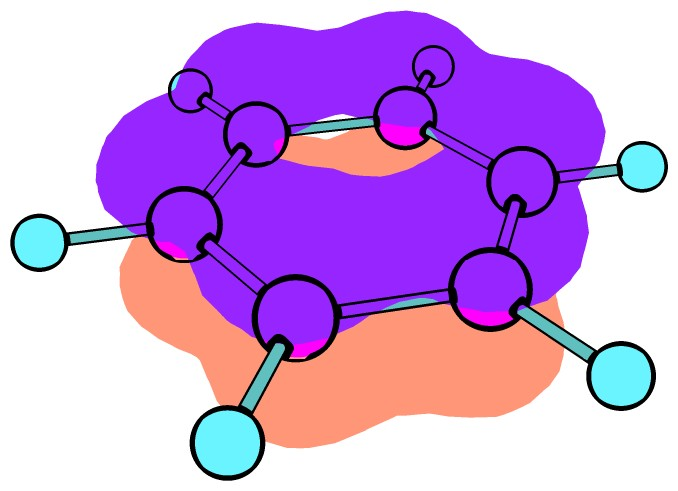
\includegraphics[scale=0.3]{fig/2.jpg}
\caption{Комплекс №1.}
\end{figure}

\begin{figure}[H]
\centering
\captionsetup{justification=centering}
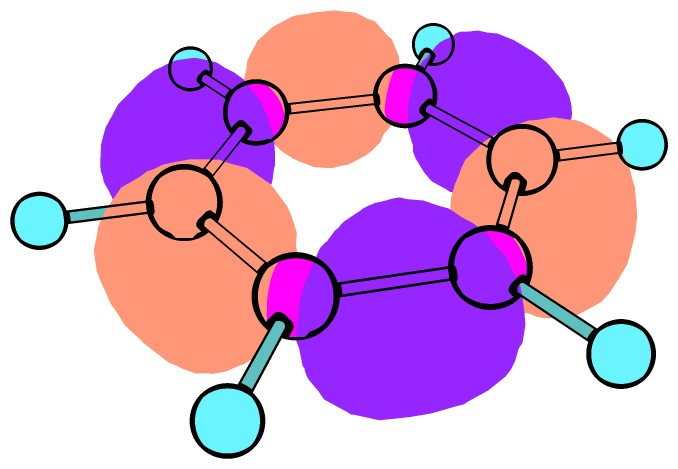
\includegraphics[scale=0.3]{fig/3.jpg}
\caption{Комплекс №2.}
\end{figure}


\subsection{Выводы}
Полученное значение энергии водородной связи для двух соединений находится в допустимом пределе: (0.003 - 0.022) Хартри. Оба комплекса являются стабильными и в растворе могут быть присутствовать оба комплекса.


\subsection{Контроль результатов}

\begin{itemize}
    \item у каждого рассматриваемого комплекса в выходном файле содержится “EQUILIBRIUM GEOMETRY LOCATED”;
    \item из пяти предложенных конформеров были обнаружены тождественные: энергия совпадает до 4 знака после запятой, геометрии тождественны; 
    \item значения энергий водородной связи находятся в допустимых пределах.
\end{itemize}{}


\subsection{Приложенные файлы}
\begin{itemize}
    \item complex\_origin.xyz – исходная структура невзаимодействующего комплекса;
    \item файлы в папке input – файлы на вход GAMESS;
    \item файлы в папке output – выходные файлы GAMESS.
\end{itemize}{}

% % Не редактируем: Страница библиографии (формируется автоматически из книжек, указанных в refs.bib и пометок \cite{имя_источника} в тексте)
% \newpage
\printbibliography[title=Перечень использованных источников]
\addcontentsline{toc}{subsection}{Перечень использованных источников}
% \end{document}
